% answers.tex —— 2004 年·全国卷Ⅳ·文科 · 参考答案与详细解析片段
% 由 tools/generate_projects.py 依来源总账自 2004/2004_数学真题_全国4文_试题.md + 2004/2004_数学真题_全国4文_解析正文.md + 2004/2004_数学真题_全国4文_答案要点.md 生成，勿手改（改源 MD 后重跑）


\begin{gktip}
固定源 PDF 为印刷页码 196–197 的两页题面，不附答案。以下解析均依据固定源独立推导复算；第 21 题图形在 LaTeX 工程中以 TikZ/PGFPlots 矢量源重绘。
\end{gktip}

\begin{answer}
\gksolhead{1}{}

\textbf{题目}：

设集合 $U=\{0,1,2,3,4,5\}$，集合 $M=\{0,3,5\}$，$N=\{1,4,5\}$，则 $M\cap(\complement_U N)=$\mbox{（　　）}

（A）$\{5\}$　　（B）$\{0,3\}$　　（C）$\{0,2,3,5\}$　　（D）$\{0,1,3,4,5\}$

\Needspace{4\baselineskip}
\textbf{解析}

全集 $U=\{0,1,2,3,4,5\}$，集合 $N=\{1,4,5\}$，
则 $\complement_U N=\{0,2,3\}$。
又集合 $M=\{0,3,5\}$，
所以 $M\cap(\complement_U N)=\{0,3\}$。
故选 B。

\gkanswer{答案：B}

\end{answer}
\begin{answer}
\gksolhead{2}{}

\textbf{题目}：

函数 $y=\mathrm{e}^{2x}$（$x\in\mathbf{R}$）的反函数为\mbox{（　　）}

（A）$y=2\ln x$（$x>0$）　　（B）$y=\ln(2x)$（$x>0$）

（C）$y=\dfrac{1}{2}\ln x$（$x>0$）　　（D）$y=\dfrac{1}{2}\ln 2x$（$x>0$）

\Needspace{4\baselineskip}
\textbf{解析}

由 $y=\mathrm{e}^{2x}$（$x\in\mathbf{R}$），
因为 $\mathrm{e}^{2x}>0$，所以 $y>0$。
两边取自然对数得 $2x=\ln y$，解得 $x=\dfrac{1}{2}\ln y$。
互换 $x,y$ 得反函数为 $y=\dfrac{1}{2}\ln x$（$x>0$）。
故选 C。

\gkanswer{答案：C}

\end{answer}
\begin{answer}
\gksolhead{3}{}

\textbf{题目}：

正三棱柱侧面的一条对角线长为 2，且与底面成 $45^\circ$ 角，则此三棱柱的体积为\mbox{（　　）}

（A）$\dfrac{\sqrt{6}}{2}$　　（B）$\sqrt{6}$　　（C）$\dfrac{\sqrt{6}}{6}$　　（D）$\dfrac{\sqrt{6}}{3}$

\Needspace{4\baselineskip}
\textbf{解析}

设正三棱柱的底面正三角形边长为 $a$，侧棱长（即柱高）为 $h$。
正三棱柱侧面为矩形，侧面对角线与底面所成的角即对角线与其在底面上投影（即底边）所成的角，
故该角为 $45^\circ$，因此侧面矩形为正方形，即 $h=a$。
\Needspace{5\baselineskip}
侧面对角线长为 2，由勾股定理得：
\nopagebreak[4]
\[
a^2+h^2=2a^2=2^2=4\implies a^2=2,\quad a=\sqrt{2},\quad h=\sqrt{2}.
\]
\Needspace{5\baselineskip}
底面正三角形的面积为：
\nopagebreak[4]
\[
S=\frac{\sqrt{3}}{4}a^2=\frac{\sqrt{3}}{4}\times 2=\frac{\sqrt{3}}{2}.
\]
\Needspace{5\baselineskip}
因此正三棱柱的体积为：
\nopagebreak[4]
\[
V=S\cdot h=\frac{\sqrt{3}}{2}\times\sqrt{2}=\frac{\sqrt{6}}{2}.
\]
故选 A。

\gkanswer{答案：A}

\end{answer}
\begin{answer}
\gksolhead{4}{}

\textbf{题目}：

函数 $y=(x+1)^2(x-1)$ 在 $x=1$ 处的导数等于\mbox{（　　）}

（A）1　　（B）2　　（C）3　　（D）4

\Needspace{4\baselineskip}
\textbf{解析}

\Needspace{5\baselineskip}
对函数 $y=(x+1)^2(x-1)$ 求导：
\nopagebreak[4]
\[
y'=2(x+1)(x-1)+(x+1)^2.
\]
将 $x=1$ 代入导数表达式：
第一项为 $2(1+1)(1-1)=0$，
第二项为 $(1+1)^2=4$。
所以 $y'\big|_{x=1}=4$。
故选 D。

\gkanswer{答案：D}

\end{answer}
\begin{answer}
\gksolhead{5}{}

\textbf{题目}：

为了得到函数 $y=3\times\left(\dfrac{1}{3}\right)^x$ 的图象，可以把函数 $y=\left(\dfrac{1}{3}\right)^x$ 的图象\mbox{（　　）}

（A）向左平移 3 个单位长度　　（B）向右平移 3 个单位长度

（C）向左平移 1 个单位长度　　（D）向右平移 1 个单位长度

\Needspace{4\baselineskip}
\textbf{解析}

\Needspace{5\baselineskip}
函数表达式可化为：
\nopagebreak[4]
\[
y=3\times\left(\frac{1}{3}\right)^x=\left(\frac{1}{3}\right)^{-1}\times\left(\frac{1}{3}\right)^x=\left(\frac{1}{3}\right)^{x-1}.
\]
根据函数图象平移变换法则“左加右减”，将函数 $y=\left(\dfrac{1}{3}\right)^x$ 的图象向右平移 1 个单位长度，自变量由 $x$ 变为 $x-1$，即可得到 $y=\left(\dfrac{1}{3}\right)^{x-1}=3\times\left(\dfrac{1}{3}\right)^x$ 的图象。
故选 D。

\gkanswer{答案：D}

\end{answer}
\begin{answer}
\gksolhead{6}{}

\textbf{题目}：

等差数列 $\{a_n\}$ 中，$a_1+a_2+a_3=-24$，$a_{18}+a_{19}+a_{20}=78$，则此数列前 20 项和等于\mbox{（　　）}

（A）160　　（B）180　　（C）200　　（D）220

\Needspace{4\baselineskip}
\textbf{解析}

\Needspace{5\baselineskip}
在等差数列 $\{a_n\}$ 中，由等差数列的性质：
\nopagebreak[4]
\[
(a_1+a_2+a_3)+(a_{18}+a_{19}+a_{20})=(a_1+a_{20})+(a_2+a_{19})+(a_3+a_{18})=3(a_1+a_{20}).
\]
已知 $a_1+a_2+a_3=-24$，$a_{18}+a_{19}+a_{20}=78$，
\Needspace{5\baselineskip}
两式相加得：
\nopagebreak[4]
\[
3(a_1+a_{20})=-24+78=54\implies a_1+a_{20}=18.
\]
\Needspace{5\baselineskip}
前 20 项和为：
\nopagebreak[4]
\[
S_{20}=\frac{20(a_1+a_{20})}{2}=10(a_1+a_{20})=10\times 18=180.
\]
故选 B。

\gkanswer{答案：B}

\end{answer}
\begin{answer}
\gksolhead{7}{}

\textbf{题目}：

已知函数 $y=\log_{\frac{1}{4}}x$ 与 $y=kx$ 的图象有公共点 $A$，且点 $A$ 的横坐标为 2，则 $k=$\mbox{（　　）}

（A）$-\dfrac{1}{4}$　　（B）$\dfrac{1}{4}$　　（C）$-\dfrac{1}{2}$　　（D）$\dfrac{1}{2}$

\Needspace{4\baselineskip}
\textbf{解析}

点 $A$ 在函数 $y=\log_{\frac{1}{4}}x$ 的图象上，且横坐标为 2，
\Needspace{5\baselineskip}
所以点 $A$ 的纵坐标为：
\nopagebreak[4]
\[
y=\log_{\frac{1}{4}}2=\log_{2^{-2}}2=-\frac{1}{2}.
\]
即 $A\left(2,-\dfrac{1}{2}\right)$。
\Needspace{5\baselineskip}
又点 $A$ 在直线 $y=kx$ 上，代入得：
\nopagebreak[4]
\[
-\frac{1}{2}=2k\implies k=-\frac{1}{4}.
\]
故选 A。

\gkanswer{答案：A}

\end{answer}
\begin{answer}
\gksolhead{8}{}

\textbf{题目}：

已知圆 $C$ 的半径为 2，圆心在 $x$ 轴的正半轴上，直线 $3x+4y+4=0$ 与圆 $C$ 相切，则圆 $C$ 的方程为\mbox{（　　）}

（A）$x^2+y^2-2x-3=0$　　（B）$x^2+y^2+4x=0$

（C）$x^2+y^2+2x-3=0$　　（D）$x^2+y^2-4x=0$

\Needspace{4\baselineskip}
\textbf{解析}

已知圆 $C$ 的圆心在 $x$ 轴正半轴上，半径 $R=2$。
设圆心坐标为 $(x_0,0)$，其中 $x_0>0$。
\Needspace{5\baselineskip}
因为直线 $3x+4y+4=0$ 与圆 $C$ 相切，所以圆心到直线的距离等于半径：
\nopagebreak[4]
\[
d=\frac{|3x_0+4\times 0+4|}{\sqrt{3^2+4^2}}=\frac{|3x_0+4|}{5}=2.
\]
从而 $|3x_0+4|=10$。
解得 $3x_0+4=10\implies x_0=2$（负值 $3x_0+4=-10\implies x_0=-\dfrac{14}{3}<0$ 舍去）。
\Needspace{5\baselineskip}
所以圆心为 $(2,0)$，半径为 2，圆的标准方程为：
\nopagebreak[4]
\[
(x-2)^2+y^2=4\implies x^2-4x+4+y^2=4\implies x^2+y^2-4x=0.
\]
故选 D。

\gkanswer{答案：D}

\end{answer}
\begin{answer}
\gksolhead{9}{}

\textbf{题目}：

从 5 位男教师和 4 位女教师中选出 3 位教师，派到 3 个班担任班主任（每班 1 位班主任），要求这 3 位班主任中男、女教师都要有，则不同的选派方案共有\mbox{（　　）}

（A）210 种　　（B）420 种　　（C）630 种　　（D）840 种

\Needspace{4\baselineskip}
\textbf{解析}

从 5 位男教师和 4 位女教师中选出 3 位担任 3 个班的班主任，每个班 1 位，属于排列问题。
\Needspace{5\baselineskip}
不考虑性别限制，不同的选派方案总数为：
\nopagebreak[4]
\[
\mathrm{A}_9^3=9\times 8\times 7=504.
\]
\Needspace{5\baselineskip}
其中，3 位班主任全为男教师的方案数为：
\nopagebreak[4]
\[
\mathrm{A}_5^3=5\times 4\times 3=60.
\]
\Needspace{5\baselineskip}
3 位班主任全为女教师的方案数为：
\nopagebreak[4]
\[
\mathrm{A}_4^3=4\times 3\times 2=24.
\]
\Needspace{5\baselineskip}
要求 3 位班主任中男、女教师都要有，排除全男和全女的情况，不同的选派方案共有：
\nopagebreak[4]
\[
504-60-24=420\text{ \text{种}}.
\]
故选 B。

\gkanswer{答案：B}

\end{answer}
\begin{answer}
\gksolhead{10}{}

\textbf{题目}：

函数 $y=2\sin\left(\dfrac{\pi}{3}-x\right)-\cos\left(\dfrac{\pi}{6}+x\right)$（$x\in\mathbf{R}$）的最小值等于\mbox{（　　）}

（A）$-3$　　（B）$-2$　　（C）$-1$　　（D）$-\sqrt{5}$

\Needspace{4\baselineskip}
\textbf{解析}

利用三角函数的诱导公式与和差化积：
注意到 $\left(\dfrac{\pi}{6}+x\right)+\left(\dfrac{\pi}{3}-x\right)=\dfrac{\pi}{2}$，
\Needspace{5\baselineskip}
所以
\nopagebreak[4]
\[
\cos\left(\frac{\pi}{6}+x\right)=\cos\left[\frac{\pi}{2}-\left(\frac{\pi}{3}-x\right)\right]=\sin\left(\frac{\pi}{3}-x\right).
\]
\Needspace{5\baselineskip}
将此式代入原函数：
\nopagebreak[4]
\[
y=2\sin\left(\frac{\pi}{3}-x\right)-\sin\left(\frac{\pi}{3}-x\right)=\sin\left(\frac{\pi}{3}-x\right).
\]
因为 $x\in\mathbf{R}$，所以 $\sin\left(\dfrac{\pi}{3}-x\right)$ 的取值范围为 $[-1,1]$。
因此函数的最小值等于 $-1$。
故选 C。

\gkanswer{答案：C}

\end{answer}
\begin{answer}
\gksolhead{11}{}

\textbf{题目}：

已知球的表面积为 $20\pi$，球面上有 $A$、$B$、$C$ 三点．如果 $AB=AC=2$，$BC=2\sqrt{3}$，则球心到平面 $ABC$ 的距离为\mbox{（　　）}

（A）1　　（B）$\sqrt{2}$　　（C）$\sqrt{3}$　　（D）2

\Needspace{4\baselineskip}
\textbf{解析}

设球的半径为 $R$。由球表面积公式 $S=4\pi R^2=20\pi$，得 $R^2=5$。
在 $\triangle ABC$ 中，$AB=AC=2$，$BC=2\sqrt{3}$。
\Needspace{5\baselineskip}
由余弦定理：
\nopagebreak[4]
\[
\cos\angle BAC=\frac{AB^2+AC^2-BC^2}{2AB\cdot AC}=\frac{2^2+2^2-(2\sqrt{3})^2}{2\times 2\times 2}=\frac{8-12}{8}=-\frac{1}{2}.
\]
所以 $\angle BAC=120^\circ$。
\Needspace{5\baselineskip}
设 $\triangle ABC$ 的外接圆半径为 $r$，由正弦定理：
\nopagebreak[4]
\[
2r=\frac{BC}{\sin\angle BAC}=\frac{2\sqrt{3}}{\sin 120^\circ}=\frac{2\sqrt{3}}{\frac{\sqrt{3}}{2}}=4\implies r=2.
\]
\Needspace{5\baselineskip}
球心到平面 $ABC$ 的距离即截面圆圆心到球心的垂直距离：
\nopagebreak[4]
\[
d=\sqrt{R^2-r^2}=\sqrt{5-2^2}=\sqrt{1}=1.
\]
故选 A。

\gkanswer{答案：A}

\end{answer}
\begin{answer}
\gksolhead{12}{}

\textbf{题目}：

$\triangle ABC$ 中，$a$、$b$、$c$ 分别为 $\angle A$、$\angle B$、$\angle C$ 的对边．如果 $a$、$b$、$c$ 成等差数列，$\angle B=30^\circ$，$\triangle ABC$ 的面积为 $\dfrac{3}{2}$，那么 $b=$\mbox{（　　）}

（A）$\dfrac{1+\sqrt{3}}{2}$　　（B）$1+\sqrt{3}$　　（C）$\dfrac{2+\sqrt{3}}{2}$　　（D）$2+\sqrt{3}$

\Needspace{4\baselineskip}
\textbf{解析}

在 $\triangle ABC$ 中，已知 $a,b,c$ 成等差数列，
所以 $a+c=2b$。
三角形面积公式为 $S=\dfrac{1}{2}ac\sin B$。
\Needspace{5\baselineskip}
已知 $\angle B=30^\circ$，$S=\dfrac{3}{2}$，代入得：
\nopagebreak[4]
\[
\frac{1}{2}ac\sin 30^\circ=\frac{1}{4}ac=\frac{3}{2}\implies ac=6.
\]
\Needspace{5\baselineskip}
由余弦定理：
\nopagebreak[4]
\[
b^2=a^2+c^2-2ac\cos B=(a+c)^2-2ac-2ac\cos 30^\circ.
\]
\Needspace{5\baselineskip}
代入 $a+c=2b$ 与 $ac=6$：
\nopagebreak[4]
\[
b^2=(2b)^2-2(6)-2(6)\times\frac{\sqrt{3}}{2}=4b^2-12-6\sqrt{3}.
\]
\Needspace{5\baselineskip}
移项整理得：
\nopagebreak[4]
\[
3b^2=12+6\sqrt{3}\implies b^2=4+2\sqrt{3}=(\sqrt{3}+1)^2.
\]
因为 $b>0$，解得 $b=\sqrt{3}+1=1+\sqrt{3}$。
故选 B。

\gkanswer{答案：B}

\end{answer}
\begin{answer}
\gksolhead{13}{}

\textbf{题目}：

$\left(x-\dfrac{1}{\sqrt{x}}\right)^8$ 展开式中 $x^5$ 的系数为 $\underline{\hspace{3cm}}$．

\Needspace{4\baselineskip}
\textbf{解析}

\Needspace{5\baselineskip}
二项式 $\left(x-\dfrac{1}{\sqrt{x}}\right)^8$ 展开式的通项为：
\nopagebreak[4]
\[
T_{r+1}=\mathrm{C}_8^r x^{8-r}\left(-\frac{1}{\sqrt{x}}\right)^r=(-1)^r\mathrm{C}_8^r x^{8-r-\frac{r}{2}}=(-1)^r\mathrm{C}_8^r x^{8-\frac{3r}{2}}.
\]
令 $8-\dfrac{3r}{2}=5$，解得 $\dfrac{3r}{2}=3\implies r=2$。
\Needspace{5\baselineskip}
代入得 $x^5$ 的系数为：
\nopagebreak[4]
\[
(-1)^2\mathrm{C}_8^2=\frac{8\times 7}{2}=28.
\]
故填 28。

\gkanswer{答案：$28$}

\end{answer}
\begin{answer}
\gksolhead{14}{}

\textbf{题目}：

已知函数 $y=\dfrac{1}{2}\sin\dfrac{x+\pi}{A}$（$A>0$）的最小正周期为 $3\pi$，则 $A=\underline{\hspace{3cm}}$．

\Needspace{4\baselineskip}
\textbf{解析}

函数表达式为 $y=\dfrac{1}{2}\sin\left(\dfrac{1}{A}x+\dfrac{\pi}{A}\right)$。
因为 $A>0$，所以 $\omega=\dfrac{1}{A}$。
\Needspace{5\baselineskip}
函数的最小正周期为：
\nopagebreak[4]
\[
T=\frac{2\pi}{\omega}=2\pi A.
\]
\Needspace{5\baselineskip}
已知周期为 $3\pi$，则：
\nopagebreak[4]
\[
2\pi A=3\pi\implies A=\frac{3}{2}.
\]
故填 $\dfrac{3}{2}$。

\gkanswer{答案：$\dfrac{3}{2}$}

\end{answer}
\begin{answer}
\gksolhead{15}{}

\textbf{题目}：

向量 $\vec{a}$、$\vec{b}$ 满足 $(\vec{a}-\vec{b})\cdot(2\vec{a}+\vec{b})=-4$，且 $|\vec{a}|=2$，$|\vec{b}|=4$，则 $\vec{a}$ 与 $\vec{b}$ 夹角的余弦值等于 $\underline{\hspace{3cm}}$．

\Needspace{4\baselineskip}
\textbf{解析}

已知 $(\vec{a}-\vec{b})\cdot(2\vec{a}+\vec{b})=-4$。
\Needspace{5\baselineskip}
展开数量积：
\nopagebreak[4]
\[
2|\vec{a}|^2+\vec{a}\cdot\vec{b}-2\vec{a}\cdot\vec{b}-|\vec{b}|^2=-4\implies 2|\vec{a}|^2-\vec{a}\cdot\vec{b}-|\vec{b}|^2=-4.
\]
\Needspace{5\baselineskip}
将 $|\vec{a}|=2$、$|\vec{b}|=4$ 代入：
\nopagebreak[4]
\[
2\times 2^2-\vec{a}\cdot\vec{b}-4^2=-4\implies 8-\vec{a}\cdot\vec{b}-16=-4\implies\vec{a}\cdot\vec{b}=-4.
\]
\Needspace{5\baselineskip}
设 $\vec{a}$ 与 $\vec{b}$ 的夹角为 $\theta$，则：
\nopagebreak[4]
\[
\cos\theta=\frac{\vec{a}\cdot\vec{b}}{|\vec{a}||\vec{b}|}=\frac{-4}{2\times 4}=-\frac{1}{2}.
\]
故填 $-\dfrac{1}{2}$。

\gkanswer{答案：$-\dfrac{1}{2}$}

\end{answer}
\begin{answer}
\gksolhead{16}{}

\textbf{题目}：

\Needspace{5\baselineskip}
设 $x,y$ 满足约束条件：
\nopagebreak[4]
\[
\begin{cases}
x+y\leqslant 1,\\
y\leqslant x,\\
y\geqslant 0,
\end{cases}
\]
则 $z=2x+y$ 的最大值是 $\underline{\hspace{3cm}}$．

\Needspace{4\baselineskip}
\textbf{解析}

\Needspace{5\baselineskip}
画出约束条件确定的可行域：
\nopagebreak[4]
\[
\begin{cases}
x+y\leqslant 1,\\
y\leqslant x,\\
y\geqslant 0.
\end{cases}
\]
各边界线的交点分别为：
1. 直线 $y=0$ 与 $y=x$ 的交点为 $(0,0)$；
2. 直线 $y=0$ 与 $x+y=1$ 的交点为 $(1,0)$；
3. 直线 $y=x$ 与 $x+y=1$ 联立解得 $\left(\dfrac{1}{2},\dfrac{1}{2}\right)$。
可行域是由点 $(0,0)$、$(1,0)$、$\left(\dfrac{1}{2},\dfrac{1}{2}\right)$ 为顶点的三角形闭区域。
目标函数为 $z=2x+y$，即直线 $y=-2x+z$。截距 $z$ 最大时，直线经过可行域最右侧的顶点 $(1,0)$。
计算各顶点处的 $z$ 值：
\begin{itemize}
\item 在 $(0,0)$ 处，$z=0$；
\item 在 $\left(\dfrac{1}{2},\dfrac{1}{2}\right)$ 处，$z=2\times\dfrac{1}{2}+\dfrac{1}{2}=\dfrac{3}{2}$；
\item 在 $(1,0)$ 处，$z=2\times 1+0=2$。
\end{itemize}
故 $z$ 的最大值是 2。
故填 2。

\gkanswer{答案：$2$}

\end{answer}
\begin{answer}
\gksolhead{17}{}

\textbf{题目}：

（本小题满分 12 分）

已知 $\alpha$ 为第二象限角，且 $\sin\alpha=\dfrac{\sqrt{15}}{4}$，求 $\dfrac{\sin\left(\alpha+\dfrac{\pi}{4}\right)}{\sin 2\alpha+\cos 2\alpha+1}$ 的值．

\Needspace{4\baselineskip}
\textbf{解析}

因为 $\alpha$ 为第二象限角，且 $\sin\alpha=\dfrac{\sqrt{15}}{4}$，
\Needspace{5\baselineskip}
所以
\nopagebreak[4]
\[
\cos\alpha=-\sqrt{1-\sin^2\alpha}=-\sqrt{1-\left(\frac{\sqrt{15}}{4}\right)^2}=-\sqrt{\frac{1}{16}}=-\frac{1}{4}.
\]
\Needspace{5\baselineskip}
由两角和的正弦公式：
\nopagebreak[4]
\[
\sin\left(\alpha+\frac{\pi}{4}\right)=\sin\alpha\cos\frac{\pi}{4}+\cos\alpha\sin\frac{\pi}{4}=\frac{\sqrt{2}}{2}(\sin\alpha+\cos\alpha).
\]
\Needspace{5\baselineskip}
由二倍角公式：
\nopagebreak[4]
\[
\sin 2\alpha=2\sin\alpha\cos\alpha,\quad \cos 2\alpha=2\cos^2\alpha-1.
\]
\Needspace{5\baselineskip}
分母化简为：
\nopagebreak[4]
\[
\sin 2\alpha+\cos 2\alpha+1=2\sin\alpha\cos\alpha+2\cos^2\alpha=2\cos\alpha(\sin\alpha+\cos\alpha).
\]
\Needspace{5\baselineskip}
因为 $\sin\alpha+\cos\alpha=\dfrac{\sqrt{15}-1}{4}\neq 0$，约去公因式 $(\sin\alpha+\cos\alpha)$ 得：
\nopagebreak[4]
\[
\frac{\sin\left(\alpha+\dfrac{\pi}{4}\right)}{\sin 2\alpha+\cos 2\alpha+1}=\frac{\dfrac{\sqrt{2}}{2}(\sin\alpha+\cos\alpha)}{2\cos\alpha(\sin\alpha+\cos\alpha)}=\frac{\sqrt{2}}{4\cos\alpha}.
\]
\Needspace{5\baselineskip}
将 $\cos\alpha=-\dfrac{1}{4}$ 代入：
\nopagebreak[4]
\[
\frac{\sqrt{2}}{4\times\left(-\dfrac{1}{4}\right)}=-\sqrt{2}.
\]

\gkanswer{答案：$-\sqrt{2}$}

\end{answer}
\begin{answer}
\gksolhead{18}{}

\textbf{题目}：

（本小题满分 12 分）

已知数列 $\{a_n\}$ 为等比数列，$a_2=6$，$a_5=162$．

（1）求数列 $\{a_n\}$ 的通项公式；

（2）设 $S_n$ 是数列 $\{a_n\}$ 的前 $n$ 项和，证明 $\dfrac{S_n\cdot S_{n+2}}{S_{n+1}^2}\leqslant 1$．

\Needspace{4\baselineskip}
\textbf{解析}

（1）设等比数列 $\{a_n\}$ 的公比为 $q$。
\Needspace{5\baselineskip}
由已知 $a_2=6$，$a_5=162$，得：
\nopagebreak[4]
\[
q^3=\frac{a_5}{a_2}=\frac{162}{6}=27\implies q=3.
\]
\Needspace{5\baselineskip}
首项为：
\nopagebreak[4]
\[
a_1=\frac{a_2}{q}=\frac{6}{3}=2.
\]
\Needspace{5\baselineskip}
所以数列 $\{a_n\}$ 的通项公式为：
\nopagebreak[4]
\[
a_n=a_1 q^{n-1}=2\cdot 3^{n-1}.
\]

\Needspace{5\baselineskip}
（2）数列 $\{a_n\}$ 的前 $n$ 项和为：
\nopagebreak[4]
\[
S_n=\frac{a_1(1-q^n)}{1-q}=\frac{2(1-3^n)}{1-3}=3^n-1.
\]
由于 $n\geqslant 1$ 时 $3^n-1>0$，所以 $S_n>0$。
要证明 $\dfrac{S_n\cdot S_{n+2}}{S_{n+1}^2}\leqslant 1$，只需证明 $S_n S_{n+2}\leqslant S_{n+1}^2$，即 $S_{n+1}^2-S_n S_{n+2}\geqslant 0$。
\Needspace{5\baselineskip}
作差计算：
\nopagebreak[4]
\[
\begin{aligned}
S_{n+1}^2-S_n S_{n+2}&=(3^{n+1}-1)^2-(3^n-1)(3^{n+2}-1)\\
&=(3^{2n+2}-2\cdot 3^{n+1}+1)-(3^{2n+2}-3^n-3^{n+2}+1)\\
&=-2\cdot 3^{n+1}+3^n+3^{n+2}\\
&=3^n(-2\times 3+1+3^2)\\
&=3^n(-6+1+9)=4\cdot 3^n.
\end{aligned}
\]
因为 $n\in\mathbf{N}^*$，所以 $4\cdot 3^n>0$ 恒成立。
\Needspace{5\baselineskip}
从而 $S_{n+1}^2>S_n S_{n+2}$，即：
\nopagebreak[4]
\[
\frac{S_n\cdot S_{n+2}}{S_{n+1}^2}<1\leqslant 1.
\]
不等式得证。

\gkanswer{答案：（1）$a_n=2\cdot 3^{n-1}$；（2）证明见解析}

\end{answer}
\begin{answer}
\gksolhead{19}{}

\textbf{题目}：

（本小题满分 12 分）

已知直线 $l_1$ 为曲线 $y=x^2+x-2$ 在点 $(1,0)$ 处的切线，$l_2$ 为该曲线的另一条切线，且 $l_1\perp l_2$．

（1）求直线 $l_2$ 的方程；

（2）求由直线 $l_1$、$l_2$ 和 $x$ 轴所围成的三角形的面积．

\Needspace{4\baselineskip}
\textbf{解析}

（1）对曲线 $y=x^2+x-2$ 求导得 $y'=2x+1$。
在点 $(1,0)$ 处的切线斜率为 $k_1=y'\big|_{x=1}=2(1)+1=3$。
\Needspace{5\baselineskip}
切线 $l_1$ 的方程为：
\nopagebreak[4]
\[
y-0=3(x-1)\implies 3x-y-3=0.
\]
\Needspace{5\baselineskip}
因为 $l_1\perp l_2$，所以切线 $l_2$ 的斜率为：
\nopagebreak[4]
\[
k_2=-\frac{1}{k_1}=-\frac{1}{3}.
\]
\Needspace{5\baselineskip}
设直线 $l_2$ 与曲线相切于点 $(x_0,y_0)$，则：
\nopagebreak[4]
\[
y'\big|_{x=x_0}=2x_0+1=-\frac{1}{3}\implies 2x_0=-\frac{4}{3}\implies x_0=-\frac{2}{3}.
\]
\Needspace{5\baselineskip}
代入曲线方程求切点纵坐标：
\nopagebreak[4]
\[
y_0=\left(-\frac{2}{3}\right)^2+\left(-\frac{2}{3}\right)-2=\frac{4}{9}-\frac{2}{3}-2=-\frac{20}{9}.
\]
\Needspace{5\baselineskip}
故切线 $l_2$ 的方程为：
\nopagebreak[4]
\[
y-\left(-\frac{20}{9}\right)=-\frac{1}{3}\left(x-\left(-\frac{2}{3}\right)\right)\implies y+\frac{20}{9}=-\frac{1}{3}x-\frac{2}{9}.
\]
\Needspace{5\baselineskip}
两边同乘 9 整理得：
\nopagebreak[4]
\[
3x+9y+22=0.
\]

（2）求直线 $l_1$、$l_2$ 分别与 $x$ 轴的交点：
在 $l_1: 3x-y-3=0$ 中，令 $y=0$ 得 $3x=3\implies x=1$，交点为 $A(1,0)$；
在 $l_2: 3x+9y+22=0$ 中，令 $y=0$ 得 $3x=-22\implies x=-\dfrac{22}{3}$，交点为 $B\left(-\dfrac{22}{3},0\right)$。
\Needspace{5\baselineskip}
线段 $AB$ 在 $x$ 轴上的长度为：
\nopagebreak[4]
\[
|AB|=1-\left(-\frac{22}{3}\right)=\frac{25}{3}.
\]
求直线 $l_1$ 与 $l_2$ 的交点 $P$：
\Needspace{5\baselineskip}
联立方程组：
\nopagebreak[4]
\[
\begin{cases}
3x-y-3=0,\\
3x+9y+22=0.
\end{cases}
\]
两式相减得 $10y+25=0\implies y=-\dfrac{5}{2}$。
\Needspace{5\baselineskip}
三角形在底边 $AB$ 上的高为交点 $P$ 到 $x$ 轴的距离：
\nopagebreak[4]
\[
h=|y_P|=\frac{5}{2}.
\]
\Needspace{5\baselineskip}
因此，由直线 $l_1$、$l_2$ 和 $x$ 轴所围成的三角形面积为：
\nopagebreak[4]
\[
S=\frac{1}{2}\times |AB|\times h=\frac{1}{2}\times\frac{25}{3}\times\frac{5}{2}=\frac{125}{12}.
\]

\gkanswer{答案：（1）$3x+9y+22=0$；（2）$\dfrac{125}{12}$}

\end{answer}
\begin{answer}
\gksolhead{20}{}

\textbf{题目}：

（本小题满分 12 分）

某同学参加科普知识竞赛，需回答 3 个问题．竞赛规则规定：答对第一、二、三问题分别得 100 分、100 分、200 分，答错得零分．假设这名同学答对第一、二、三个问题的概率分别为 0.8、0.7、0.6，且各题答对与否相互之间没有影响．

（1）求这名同学得 300 分的概率；

（2）求这名同学至少得 300 分的概率．

\Needspace{4\baselineskip}
\textbf{解析}

记该同学答对第 1、2、3 个问题的事件分别记为 $A_1$、$A_2$、$A_3$。
\Needspace{5\baselineskip}
由题意，$A_1,A_2,A_3$ 相互独立，且
\nopagebreak[4]
\[
P(A_1)=0.8,\quad P(A_2)=0.7,\quad P(A_3)=0.6,
\]
\Needspace{5\baselineskip}
答错各题的概率分别为：
\nopagebreak[4]
\[
P(\bar{A}_1)=1-0.8=0.2,\quad P(\bar{A}_2)=1-0.7=0.3,\quad P(\bar{A}_3)=1-0.6=0.4.
\]
答对第一、二、三题得分分别为 100 分、100 分、200 分。

（1）该同学得 300 分，只有以下两种互斥情况：
\begin{itemize}
\item 答对第 1 题和第 3 题，答错第 2 题，此时得分为 $100+0+200=300$ 分，概率为：
\end{itemize}
\nopagebreak[4]
\[
P_1=P(A_1\bar{A}_2 A_3)=0.8\times(1-0.7)\times 0.6=0.8\times 0.3\times 0.6=0.144;
\]
\begin{itemize}
\item 答错第 1 题，答对第 2 题和第 3 题，此时得分为 $0+100+200=300$ 分，概率为：
\end{itemize}
\nopagebreak[4]
\[
P_2=P(\bar{A}_1 A_2 A_3)=(1-0.8)\times 0.7\times 0.6=0.2\times 0.7\times 0.6=0.084.
\]
\Needspace{5\baselineskip}
所以该同学得 300 分的概率为：
\nopagebreak[4]
\[
P=P_1+P_2=0.144+0.084=0.228.
\]

（2）该同学可能获得的满分为 $100+100+200=400$ 分。
因此“至少得 300 分”包含“得 300 分”与“得 400 分”两种互斥情形。
\Needspace{5\baselineskip}
得 400 分即 3 个问题全部答对，概率为：
\nopagebreak[4]
\[
P(400)=P(A_1 A_2 A_3)=0.8\times 0.7\times 0.6=0.336.
\]
\Needspace{5\baselineskip}
因此该同学至少得 300 分的概率为：
\nopagebreak[4]
\[
P(\text{\text{至少得} }300\text{ \text{分}})=P(300)+P(400)=0.228+0.336=0.564.
\]

\gkanswer{答案：（1）$0.228$；（2）$0.564$}

\end{answer}
\begin{answer}
\gksolhead{21}{}

\textbf{题目}：

（本小题满分 12 分）

如图，四棱锥 $P-ABCD$ 中，底面 $ABCD$ 为矩形，$AB=8$，$AD=4\sqrt{3}$，侧面 $PAD$ 为等边三角形，并且与底面所成二面角为 $60^\circ$．
\nopagebreak[4]
\begin{center}% 2004 年全国卷Ⅳ文科第 21 题：四棱锥立体几何图
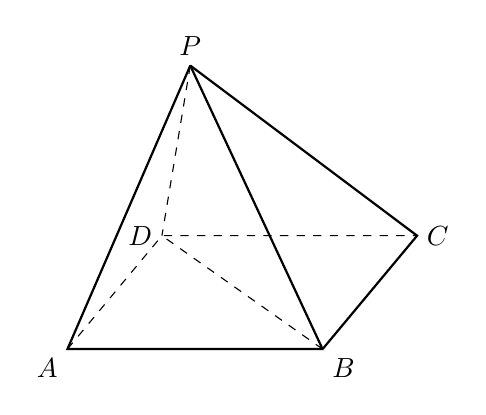
\begin{tikzpicture}[>=stealth,scale=1.2]
  % Coordinates
  \coordinate (A) at (-1.5,-0.8);
  \coordinate (B) at (1.2,-0.8);
  \coordinate (C) at (2.2,0.4);
  \coordinate (D) at (-0.5,0.4);
  \coordinate (P) at (-0.2,2.2);

  % Solid edges
  \draw[thick] (P) -- (A) -- (B) -- (C) -- (P);
  \draw[thick] (P) -- (B);

  % Dashed edges
  \draw[dashed] (A) -- (D) -- (C);
  \draw[dashed] (P) -- (D);
  \draw[dashed] (B) -- (D);

  % Labels
  \node[below left] at (A) {$A$};
  \node[below right] at (B) {$B$};
  \node[right] at (C) {$C$};
  \node[left] at (D) {$D$};
  \node[above] at (P) {$P$};
\end{tikzpicture}
\end{center}
\nopagebreak[4]
（1）求四棱锥 $P-ABCD$ 的体积；

（2）证明：$PA\perp BD$．

\Needspace{4\baselineskip}
\textbf{解析}

（1）在四棱锥 $P-ABCD$ 中，底面 $ABCD$ 为矩形，$AB=8$，$AD=4\sqrt{3}$。
侧面 $PAD$ 为等边三角形，其边长为 $AD=4\sqrt{3}$。
取 $AD$ 的中点为 $E$，连接 $PE$。
\Needspace{5\baselineskip}
在等边 $\triangle PAD$ 中，$PE\perp AD$，且
\nopagebreak[4]
\[
PE=\frac{\sqrt{3}}{2}AD=\frac{\sqrt{3}}{2}\times 4\sqrt{3}=6.
\]
过点 $P$ 作底面 $ABCD$ 的垂线，垂足为 $H$。
因为 $PE\perp AD$，$PH\perp\text{\text{底面} }ABCD$，由三垂线定理的逆定理可知 $EH\perp AD$。
所以 $\angle PEH$ 即为侧面 $PAD$ 与底面 $ABCD$ 所成二面角的平面角，
已知该二面角为 $60^\circ$，即 $\angle PEH=60^\circ$。
在 $\text{Rt}\triangle PHE$ 中：
\Needspace{5\baselineskip}
四棱锥的高为：
\nopagebreak[4]
\[
h=PH=PE\sin 60^\circ=6\times\frac{\sqrt{3}}{2}=3\sqrt{3}.
\]
\Needspace{5\baselineskip}
矩形底面 $ABCD$ 的面积为：
\nopagebreak[4]
\[
S_{ABCD}=AB\times AD=8\times 4\sqrt{3}=32\sqrt{3}.
\]
\Needspace{5\baselineskip}
因此，四棱锥 $P-ABCD$ 的体积为：
\nopagebreak[4]
\[
V=\frac{1}{3}S_{ABCD}\cdot h=\frac{1}{3}\times 32\sqrt{3}\times 3\sqrt{3}=96.
\]

\Needspace{5\baselineskip}
（2）在 $\text{Rt}\triangle PHE$ 中，
\nopagebreak[4]
\[
EH=PE\cos 60^\circ=6\times\frac{1}{2}=3.
\]
在底面矩形 $ABCD$ 中，$AB\perp AD$ 且 $EH\perp AD$，所以 $EH\parallel AB$。
因为侧面 $PAD$ 与底面所成二面角为锐角 $60^\circ$，垂足 $H$ 落在底面矩形内部。
以 $A$ 为原点，射线 $AD$ 为 $x$ 轴正半轴，射线 $AB$ 为 $y$ 轴正半轴，过 $A$ 点垂直于底面向上为 $z$ 轴正半轴建立空间直角坐标系。
\Needspace{5\baselineskip}
由题设各点坐标为：
\nopagebreak[4]
\[
A(0,0,0),\quad D(4\sqrt{3},0,0),\quad B(0,8,0),\quad C(4\sqrt{3},8,0).
\]
因为 $E$ 为 $AD$ 中点，所以 $E(2\sqrt{3},0,0)$。
点 $H$ 在底面内，满足 $EH\parallel AB$ 且 $EH=3$，故 $H(2\sqrt{3},3,0)$。
\Needspace{5\baselineskip}
因为 $PH\perp\text{\text{底面}}$ 且 $PH=3\sqrt{3}$，所以顶点 $P$ 的坐标为：
\nopagebreak[4]
\[
P(2\sqrt{3},3,3\sqrt{3}).
\]
\Needspace{5\baselineskip}
从而有向量：
\nopagebreak[4]
\[
\vec{PA}=\vec{OA}-\vec{OP}=(-2\sqrt{3},-3,-3\sqrt{3}),
\]
\nopagebreak[4]
\[
\vec{BD}=\vec{OD}-\vec{OB}=(4\sqrt{3},-8,0).
\]
\Needspace{5\baselineskip}
计算数量积：
\nopagebreak[4]
\[
\vec{PA}\cdot\vec{BD}=(-2\sqrt{3})\times(4\sqrt{3})+(-3)\times(-8)+(-3\sqrt{3})\times 0=-24+24+0=0.
\]
因为 $\vec{PA}\cdot\vec{BD}=0$，所以 $\vec{PA}\perp\vec{BD}$。
即 $PA\perp BD$。

\gkanswer{答案：（1）$96$；（2）证明见解析}

\end{answer}
\begin{answer}
\gksolhead{22}{}

\textbf{题目}：

（本小题满分 14 分）

双曲线 $\dfrac{x^2}{a^2}-\dfrac{y^2}{b^2}=1$（$a>1,b>0$）的焦点距为 $2c$，直线 $l$ 过点 $(a,0)$ 和 $(0,b)$，且点 $(1,0)$ 到直线 $l$ 的距离与点 $(-1,0)$ 到直线 $l$ 的距离之和 $s\geqslant\dfrac{4}{5}c$．求双曲线的离心率 $e$ 的取值范围．

\Needspace{4\baselineskip}
\textbf{解析}

双曲线的标准方程为 $\dfrac{x^2}{a^2}-\dfrac{y^2}{b^2}=1$（$a>1,b>0$），焦点距为 $2c$，则 $c^2=a^2+b^2$。
直线 $l$ 过点 $(a,0)$ 和 $(0,b)$，其截距式方程为 $\dfrac{x}{a}+\dfrac{y}{b}=1$，
\Needspace{5\baselineskip}
化为一般式方程为：
\nopagebreak[4]
\[
bx+ay-ab=0.
\]
由点到直线的距离公式：
\Needspace{5\baselineskip}
点 $(1,0)$ 到直线 $l$ 的距离为：
\nopagebreak[4]
\[
d_1=\frac{|b\cdot 1+a\cdot 0-ab|}{\sqrt{a^2+b^2}}=\frac{|b-ab|}{c}=\frac{b|1-a|}{c}.
\]
\Needspace{5\baselineskip}
因为 $a>1$，所以 $|1-a|=a-1$，即
\nopagebreak[4]
\[
d_1=\frac{b(a-1)}{c}.
\]
\Needspace{5\baselineskip}
点 $(-1,0)$ 到直线 $l$ 的距离为：
\nopagebreak[4]
\[
d_2=\frac{|b\cdot(-1)+a\cdot 0-ab|}{\sqrt{a^2+b^2}}=\frac{|-b-ab|}{c}=\frac{b(a+1)}{c}.
\]
\Needspace{5\baselineskip}
因此两点到直线 $l$ 的距离之和为：
\nopagebreak[4]
\[
s=d_1+d_2=\frac{b(a-1)+b(a+1)}{c}=\frac{2ab}{c}.
\]
\Needspace{5\baselineskip}
已知 $s\geqslant\dfrac{4}{5}c$，即
\nopagebreak[4]
\[
\frac{2ab}{c}\geqslant\frac{4}{5}c\implies ab\geqslant\frac{2}{5}c^2.
\]
\Needspace{5\baselineskip}
两边同除以 $c^2$：
\nopagebreak[4]
\[
\frac{a}{c}\cdot\frac{b}{c}\geqslant\frac{2}{5}.
\]
由双曲线离心率的定义 $e=\dfrac{c}{a}>1$，可得 $\dfrac{a}{c}=\dfrac{1}{e}$。
\Needspace{5\baselineskip}
又由 $b^2=c^2-a^2$，得：
\nopagebreak[4]
\[
\frac{b}{c}=\sqrt{1-\frac{a^2}{c^2}}=\sqrt{1-\frac{1}{e^2}}=\frac{\sqrt{e^2-1}}{e}.
\]
\Needspace{5\baselineskip}
将此代入不等式中：
\nopagebreak[4]
\[
\frac{1}{e}\cdot\frac{\sqrt{e^2-1}}{e}\geqslant\frac{2}{5}\implies\frac{\sqrt{e^2-1}}{e^2}\geqslant\frac{2}{5}.
\]
\Needspace{5\baselineskip}
因为 $e>1$，两边平方得：
\nopagebreak[4]
\[
\frac{e^2-1}{e^4}\geqslant\frac{4}{25}.
\]
\Needspace{5\baselineskip}
令 $t=e^2$（$t>1$），不等式化为：
\nopagebreak[4]
\[
\frac{t-1}{t^2}\geqslant\frac{4}{25}\implies 4t^2-25t+25\leqslant 0.
\]
\Needspace{5\baselineskip}
因式分解：
\nopagebreak[4]
\[
(4t-5)(t-5)\leqslant 0.
\]
\Needspace{5\baselineskip}
解得：
\nopagebreak[4]
\[
\frac{5}{4}\leqslant t\leqslant 5\implies\frac{5}{4}\leqslant e^2\leqslant 5.
\]
\Needspace{5\baselineskip}
因为 $e>1$，所以
\nopagebreak[4]
\[
\frac{\sqrt{5}}{2}\leqslant e\leqslant\sqrt{5}.
\]
因此，双曲线的离心率 $e$ 的取值范围是 $\left[\dfrac{\sqrt{5}}{2},\sqrt{5}\right]$。

\gkanswer{答案：$\left[\dfrac{\sqrt{5}}{2}, \sqrt{5}\right]$}

\end{answer}